\chapter{数据}
\section{期权数据}
\par{    
本文主要采用期权交易所LedgerX(https://www.ledgerx.com)公开的每日交易数据,数据位于其网站的“数据”栏目上(data.ledgerx.com),该交易所的所有期权均为欧式期权。数据包括期权合约条款(行权价、是否为认购、到期日)、每日成交量加权平均价、成交量、持仓量、最后一次买价和卖价等。其中一天的数据示例如下图所示:
\begin{figure}[H]
\begin{small}
\begin{center}
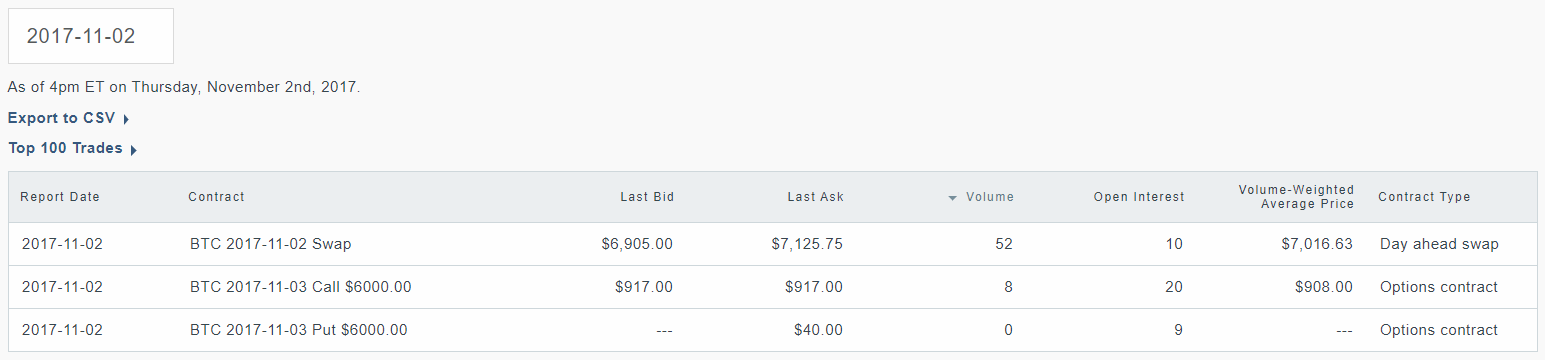
\includegraphics[width=0.95\textwidth]{figures/data_example.png}
\end{center}
\caption{LedgerX数据展示}
\label{data_example}
\end{small}
\end{figure}
利用python爬虫获取了2017年10月17日至2018年12月31日的全部数据,剔除了如图\ref{data_example}中所示的隔夜互换、交易量为0(只有买价或卖价)的数据之后,得到共计1726条期权的交易数据。然而根据Black和Scholes(1972)\cite{J-1972}以及Macbeth和Merville(1979)\cite{Jame-1979}两次利用期权定价模型进行的实证研究,一般认为离到期日较近的期权、价值更虚的期权往往定价不准确,因此之后进行回归时会做进一步筛选。期权数据的成交量加权平均价可被认为是当天该期权的平均成交价格水平,故后文提到的“市场价格”均指该期权的成交量加权平均价。
} 

\par{
将期权交易数据按照其标签(即合约的到期日、行权价、认购/认沽方向)分组,并对基本信息统计如下:
}
\par{
\begin{center}
\begin{threeparttable}[H]
\centering
\caption{期权信息描述性统计}
\label{option_describe}
\begin{tabular}{lrrrr}
\toprule
{} &      期限 &       行权价 &  认购期权数量 &  认沽期权数量 \\
\midrule
count & 306.000 &   306.000 & 197.000 & 109.000 \\
mean  &  90.536 &  8867.647 &         &         \\
std   & 141.132 &  6207.192 &         &         \\
min   &   1.000 &  2000.000 &         &         \\
25\%   &   3.250 &  6000.000 &         &         \\
50\%   &  30.000 &  7000.000 &         &         \\
75\%   &  96.750 & 10000.000 &         &         \\
max   & 637.000 & 50000.000 &         &         \\
\bottomrule
\end{tabular}

\begin{tablenotes}
\footnotesize
\item 注:此处统计已将期权按照到期日、行权价和方向分组。期限为第一个有交易的日期至到期日的天数。
\end{tablenotes}
\end{threeparttable}
\end{center}
}
~\\
\par{
从表\ref{option_describe}可见,认购期权种类略多于认沽期权,目前期权的行权价覆盖范围已经较广,从2000元-50000元均有期权。对期权的期限而言,有50$\%$位于30天以下,此外存在一部分期限极短的数据,可能存在之前无交易的情况。另一方面,根据Black和Scholes(1972,1973)\cite{J-1972}\cite{10.2307/1831029},Macbeth和Merville(1979)\cite{Jame-1979},深度价外期权和期限较短的期权并不适合用B-S模型定价。因此我们对数据做如下清理:
\begin{itemize}
    \item 剔除每日交易量仅有1的记录。
    \item 剔除距离到期日在7日之内的记录。
    \item 剔除认购期权的相对价值在0.8以下,认沽期权的相对价值在1.25以上的记录(相对价值定义为比特币市场价与期权行权价之比)。
    
\end{itemize}
}
\section{比特币数据}

\par{为保证之后回归的准确和套利策略的可行性,我们选择coinmarketcap网站(https://coinmarketcap.com)上公开的各美元交易所的比特币加权均价,这样可以保证以交易量较大的比特币交易所价格为基础,作为套利策略应用价格较为可行。
比特币有众多交易所,根据Makarov(2018)可知,不同交易所之间价格存在一定差异,且用不同货币交易的交易所之间套利空间更为巨大\cite{Makarov-2018},考虑到期权行权和交易均以美元报价,这里我们限制选择以美元为交易货币的交易所,构建与这一文献中类似的套利指数。根据比特币数据汇总网站Bitcoinity(https://bitcoinity.org)提供数据,可得到所有美元交易所中,每日结算价中最高者和最低者之比。图\ref{maxmin_ratio}分别展示了数据期内比特币价格、成交量走势、波动率(一年滚动窗口)和比值走势:
\begin{figure}[H]
\begin{small}
    \begin{center}
        \includegraphics[width=1\textwidth]{figures/maxmin_ratio_plot.png} 
    \end{center}
    \caption{比特币加权均价走势与交易所间最高价与最低价之比}
    \label{maxmin_ratio}
\end{small}
\end{figure}
}
\par{比特币交易所之间的价格差异与比特币的价格和交易量有较明显的同步性。这一点与Makarov(2018)中的发现相符\cite{Makarov-2018}。这一套利空间实际上受到了不同交易所交易量的异质波动的较大影响,故交易量的提升反而会加大套利的空间。}
\par{同样根据Makarov(2018),这一套利指数实际上综合反映了噪声投资者的比例以及投资者实现套利的意愿和难易程度,比如政策风险、套利成本等因素,根据Shiller等(1984),噪声投资者比例以及套利空间是非流动性的重要测度,故这一套利指数能够被用作衡量市场流动性的解释变量。}

\par{除了价格信息之外,各种期权定价模型均需要有无风险利率信息,而比特币市场上并无公开的无风险利率。根据2015年出版的《比特币手册(Bitcoin Handbook)》\cite{WESNER2015223},作者提出了通过宏观经济理论推断比特币无风险利率的方法,根据其提供的结果,可得比特币的无风险利率在4$\%$到6$\%$之间,故取比特币无风险利率为5$\%$(年化复利)。
}


\par{
对数据搜集期比特币每日收盘价数据取对数收益率,按照一年滚动窗口计算其波动率、偏度、峰度。对其描述性统计如下:}
\begin{center}
\begin{threeparttable}[H]
    
    \centering
    \caption{比特币数据描述性统计}
    \label{btc_describe}
    \begin{tabular}{lrrrrr}
\toprule
{} &             成交量 &   对数收益率 &     波动率 &      偏度 &      峰度 \\
\midrule
count &         544.000 & 544.000 & 544.000 & 544.000 & 544.000 \\
mean  &  6749637776.700 &  -0.000 &   0.047 &  -0.096 &   2.667 \\
std   &  3790972106.645 &   0.044 &   0.007 &   0.189 &   0.802 \\
min   &  1403920000.000 &  -0.185 &   0.032 &  -0.541 &   1.656 \\
25\%   &  4273417520.000 &  -0.017 &   0.043 &  -0.313 &   2.135 \\
50\%   &  5470000143.500 &   0.002 &   0.049 &  -0.041 &   2.326 \\
75\%   &  7810741265.500 &   0.018 &   0.054 &   0.060 &   3.032 \\
max   & 23840899072.000 &   0.225 &   0.055 &   0.175 &   5.026 \\
\bottomrule
\end{tabular}

    \begin{tablenotes}
        \footnotesize
        \item 注:波动率、偏度、峰度用一年(365天)滚动窗口估计,均为日化数据;偏度为超额偏度;成交量为亿美元;数据保留三位小数。
    \end{tablenotes}
\end{threeparttable}
\end{center}

~\\
\par{

由表\ref{btc_describe}可见,数据期比特币存在一定的负偏度与高峰度。其中峰度一直保持在0以上,说明比特币收益率存在尖峰厚尾现象,而偏度数据相对波动较大,总体上比较接近0偏度,同时对数收益率均值也非常接近0,说明比特币的收益分布非常接近存在尖峰厚尾现象的对称分布。
}
